\chapter{Daten}

\section{Datenstrukturen zur Persistenz eines Neuronalen Netzes}

Jedes Neuronale Netz wird zur Persistenz auf die unten dargestellten Datenstrukturen abgebildet, welche dann in der MongoDB abgelegt werden. 
\begin{figure}[h]
\begin{center}
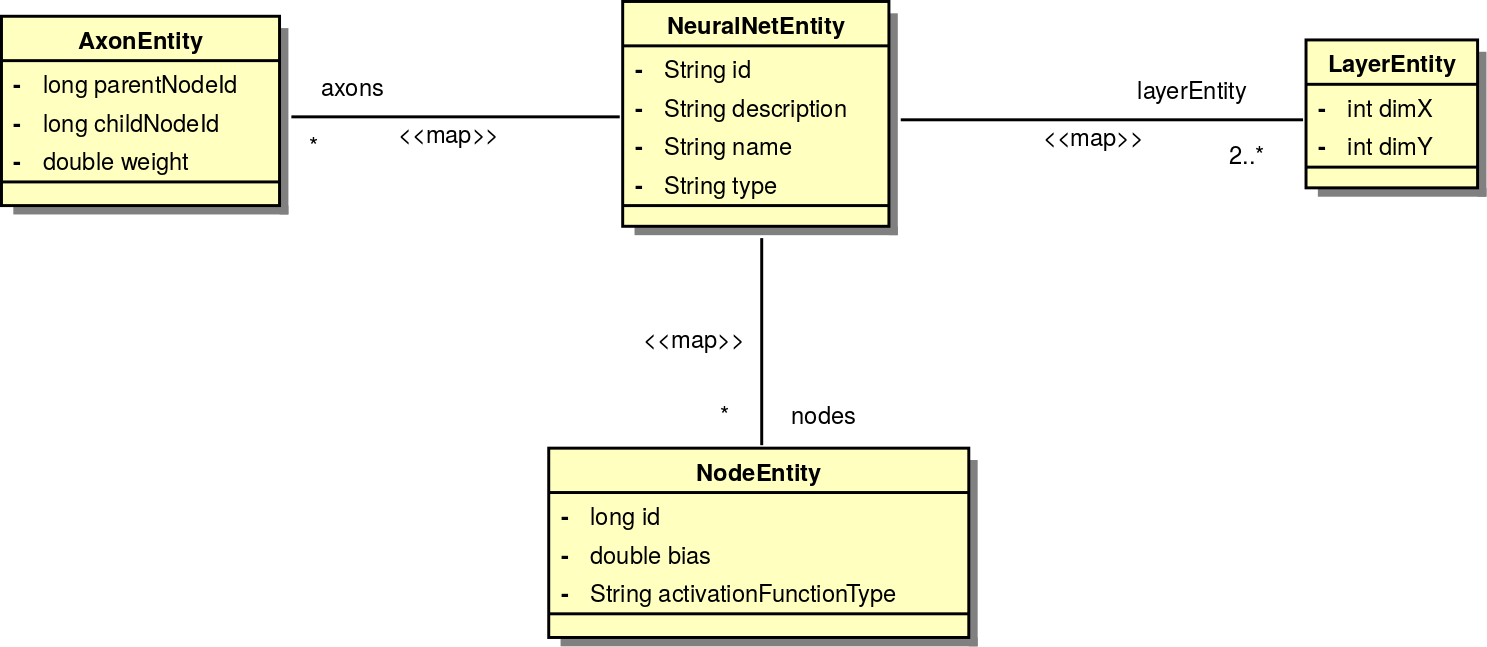
\includegraphics[width=\textwidth]{Abbildungen/UML/jan/datenBankKlassendiagramm.png}
\end{center}
\end{figure}
Es ist zu beachten, dass die Objekt dabei nicht als unabhängige, in Beziehung stehende Entitäten\footnote{Dies entspräche dem Vorgehen für eine Relationale Datenbank. Durch die vielen zirkulären Referenzen ist dieser Zugang nicht geeignet} in der Datenbank sondern als ein einziges Json-Objekt abgelegt werden. 
